\documentclass[tikz, border=8pt]{standalone}
\usepackage[T1]{fontenc}
\usepackage{tgpagella}
\usepackage{mathpazo}
\usepackage{tikz}
\usepackage{amsmath}
\usepackage{amssymb}
\usepackage{xcolor}
\usepackage{fontawesome5}
\usetikzlibrary{positioning, arrows.meta, shapes.geometric, fit, backgrounds, calc}

% ----------------------------------------------------------------
% Inline palette -- mirrors figures/_palette.tex (AGENTS.md rule 1).
% Kept inline so this figure compiles stand-alone regardless of
% TEXINPUTS, matching figures/architecture.tex.
% ----------------------------------------------------------------
\definecolor{cAudio}{HTML}{F5EFE3}
\definecolor{cEnc}{HTML}{DDE9EC}
\definecolor{cEncB}{HTML}{2D8294}
\definecolor{cAdp}{HTML}{F0DFC9}
\definecolor{cAdpB}{HTML}{B07849}
\definecolor{cLLM}{HTML}{F4E6D5}
\definecolor{cLLMB}{HTML}{A0763C}
\definecolor{cPrompt}{HTML}{F1ECE3}
\definecolor{cPromptB}{HTML}{8E7A55}
\definecolor{cTok}{HTML}{E5EEF0}
\definecolor{cTokB}{HTML}{5E8090}
\definecolor{cBound}{HTML}{ECDFD3}
\definecolor{cBoundB}{HTML}{9C7558}
\definecolor{cAuT}{HTML}{F6E1CF}
\definecolor{cAuTB}{HTML}{C77F45}

\newcommand{\frozenIcon}{\textcolor{cEncB}{\faSnowflake}}
\newcommand{\fireIcon}{\textcolor{cLLMB!90!red}{\faFire}}

\newcommand{\WaveformPictogram}{%
  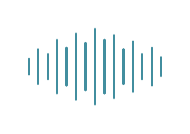
\begin{tikzpicture}[baseline=-0.6ex]
    \foreach \i/\h in {%
        0/0.10, 1/0.22, 2/0.16, 3/0.34, 4/0.24,
        5/0.42, 6/0.30, 7/0.48, 8/0.34, 9/0.40,
        10/0.22, 11/0.32, 12/0.16, 13/0.24, 14/0.12%
    }{
      \pgfmathsetmacro{\xpos}{-0.84 + \i*0.12}
      \draw[line width=0.85pt, line cap=round, draw=cEncB!90]
        (\xpos, -\h) -- (\xpos, \h);
    }
  \end{tikzpicture}%
}

\tikzset{
  box/.style       ={draw, rounded corners=3pt, align=center,
                     font=\small, line width=0.7pt,
                     minimum width=3.0cm, minimum height=1.0cm},
  frozenbox/.style ={box, fill=cEnc, draw=cEncB},
  trainbox/.style  ={box, fill=cAuT, draw=cAuTB},
  scorebox/.style  ={box, fill=cAdp!45, draw=cAdpB,
                     minimum width=4.9cm, minimum height=1.1cm},
  asrbox/.style    ={box, fill=cLLM, draw=cLLMB, line width=0.85pt,
                     minimum width=4.9cm, minimum height=1.2cm},
  poolcyl/.style   ={draw=cAdpB, fill=cAdp, line width=0.75pt,
                     cylinder, shape border rotate=90, aspect=0.25,
                     minimum width=2.1cm, minimum height=1.45cm,
                     align=center, font=\small},
  audiobox/.style  ={box, fill=cAudio, draw=black!35, minimum height=1.0cm},
  outbox/.style    ={box, fill=white, draw=black!50, minimum height=0.85cm},
  % ---- muted dashed styles for the right-hand contrast panel ----
  mbox/.style      ={box, fill=black!3, draw=black!45, dashed,
                     line width=0.6pt, text=black!70},
  mpool/.style     ={poolcyl, fill=black!4, draw=black!45, dashed,
                     line width=0.6pt, minimum width=1.7cm,
                     minimum height=1.2cm},
  maudio/.style    ={audiobox, fill=black!3, draw=black!40, dashed},
  mout/.style      ={outbox, fill=black!3, draw=black!45, dashed, text=black!70},
  flow/.style      ={-Stealth, line width=0.7pt, draw=black!70},
  mflow/.style     ={-Stealth, line width=0.65pt, draw=black!45, dashed},
  edgelabel/.style ={font=\scriptsize, text=black!55, fill=white, inner sep=1.5pt},
  medgelabel/.style={font=\scriptsize, text=black!45, fill=white, inner sep=1.5pt},
  paneltitle/.style={font=\bfseries\small, align=center, text=cLLMB},
  mtitle/.style    ={font=\bfseries\small, align=center, text=black!50},
}

\begin{document}
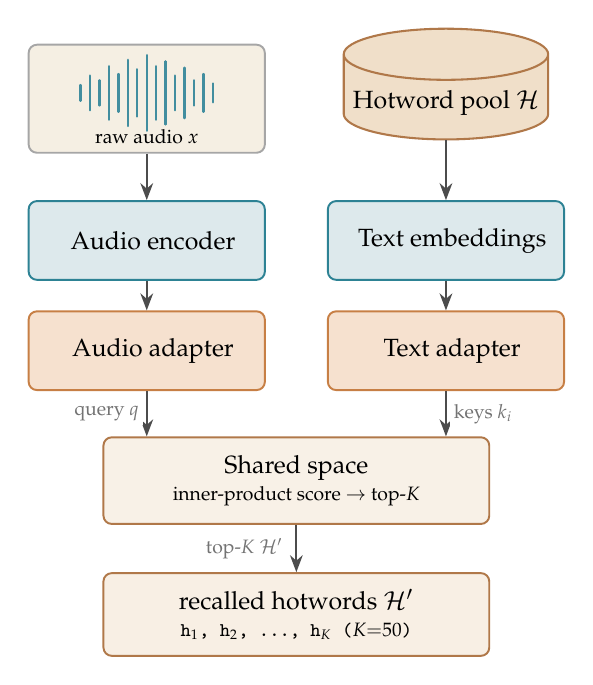
\begin{tikzpicture}

  % ============================================================
  % LEFT PANEL -- Tower retrieve-then-bias (this work)
  % Two adapters project frozen acoustic / text features into a
  % shared 512-d space; inner-product top-K feeds a single ASR pass.
  % ============================================================
  \def\xA{-1.9}   % audio-tower column
  \def\xT{1.9}    % text-tower column

  % --- audio tower ---
  \node[audiobox]  (wave) at (\xA, 6.00)
    {\WaveformPictogram\\[-2pt]{\scriptsize raw audio $x$}};
  \node[frozenbox] (aenc) at (\xA, 4.20) {\frozenIcon~~Audio encoder};
  \node[trainbox]  (aadp) at (\xA, 2.80) {\fireIcon~~Audio adapter};

  % --- text tower ---
  \node[poolcyl, minimum height=1.1cm] (pool) at (\xT, 5.95)
    {Hotword pool $\mathcal{H}$};
  \node[frozenbox] (temb) at (\xT, 4.20) {\frozenIcon~~Text embeddings};
  \node[trainbox]  (tadp) at (\xT, 2.80) {\fireIcon~~Text adapter};

  % --- shared space + single LLM pass ---
  \node[scorebox] (score) at (0, 1.15)
    {Shared space\\[-1pt]
     {\scriptsize inner-product score $\to$ top-$K$}};
  \node[box, fill=cAdp!50, draw=cAdpB,
        minimum width=4.9cm, minimum height=1.05cm] (hw) at (0, -0.55)
    {recalled hotwords $\mathcal{H}'$\\[-1pt]
     {\scriptsize\ttfamily h$_1$, h$_2$, \ldots, h$_K$ ($K{=}50$)}};

  % --- arrows (all orthogonal) ---
  \draw[flow] (wave) -- (aenc);
  \draw[flow] (aenc) -- (aadp);
  \draw[flow] (pool) -- (temb);
  \draw[flow] (temb) -- (tadp);
  \draw[flow] (aadp.south) -- (aadp.south |- score.north)
        node[midway, edgelabel, left=1pt] {query $q$};
  \draw[flow] (tadp.south) -- (tadp.south |- score.north)
        node[midway, edgelabel, right=1pt] {keys $k_i$};
  \draw[flow] (score) -- (hw)
        node[midway, edgelabel, left=3pt] {top-$K$ $\mathcal{H}'$};

\end{tikzpicture}
\end{document}
